%\section{Empirical Validation}
\subsection{Experimental Evaluation}
\label{sec:evaluation}

In this section, we first describe our experimental setup, followed by indicative examples of map-based visualizations of real-world geolocated time series, as well as scalability results using a synthetic dataset containing 4 million time series. The experiments were conducted on a Dell PowerEdge M910 with 4 Intel Xeon E7-4830 CPUs, each containing 8 cores clocked at 2.13GHz, 256 GB RAM and a total storage space of 900 GB. Finally, we assume that the index fits in memory.

\subsubsection{Experimental Setup}
\label{subsec:exp_setup}

\paragraph{Datasets}

We use two real-world datasets selected from different application domains and with diverse characteristics. In addition, we generated a synthetic dataset to test the scalability of our method. Table \ref{tab:datasets} lists a summary of the characteristics of each dataset.

%\vspace{-5pt}
\begin{table}[!h]
	\centering
	\caption{Datasets used in the experiments.}
	\vspace{-10pt}
	\begin{small}
	\centering
%	\resizebox{\linewidth}{!}{
	\begin{tabular}{lcccccc}
	\hline
	\multirow{2}{*}{Dataset} & Area & Number of & Length $w$ of \\
	 & (km$^2$) & time series & each time series \\
	\hline
	Water & 114 & 822 & 168 \\
	Taxi & 2,500 & 417,960 & 168 \\
	Synthetic & 114 & 4,000,000 & 168 \\
	\hline
	\end{tabular}
	%}
	\end{small}
	\label{tab:datasets}
\end{table}
%\vspace{-5pt}

\emph{DAIAD Water Consumption (Water)}. Courtesy of the DAIAD project, we acquired a geolocated time series dataset of hourly water consumption for 822 households in Alicante, Spain from 1/1/2015 to 20/1/2017. In order to get a more representative dataset for our tests, we calculated the average weekly time series per household, which is the average consumption value per hour of the week. Thus, the length of each resulting time series is $24 \times 7=168$ values across the week.

\emph{NYC taxi dropoffs (Taxi)}. This dataset contains time series extracted from yellow taxi rides in New York City during 2015. The original data\footnote{\url{http://www.nyc.gov/html/tlc/html/about/trip_record_data.shtml}} provide pick-up and drop-off locations, as well as corresponding timestamps for each ride. For each month, we generated time series by applying a uniform spatial grid over the entire city (cell side was 200 meters) and counting all drop-offs therein for each day of the week at the time granularity of one hour. Thus, we obtained the number of drop-offs for $24 \times 7$ time intervals in every cell, which essentially captures the weekly fluctuation of taxi destinations there. The centroid of each cell is used as the geolocation of the corresponding time series.

\emph{Synthetic Water Consumption (Synthetic)}. To examine the scalability of our method, we generated a synthetic dataset comprising 4 million geolocated time series by inflating the water consumption dataset. This was achieved by using the original time series as seeds and introducing some random variations in their location and pattern. We chose the water dataset so as to generate a more densely populated dataset (Alicante is a medium-sized city), in order to stress-test our visualization method.

\paragraph{Parameters}

We built the BTSR-Tree index setting the minimum and maximum number of entries per node to $m=60$ and $M=200$, respectively. Regarding the number of bundles, we set $k_0 = 5$ for its leaf nodes. The number of bundles for the traversal algorithm is set to be equal to the number of bundles at the leafs, i.e., $k = k_0 = 5$. For an evaluation of the BTSR-Tree index under different parameter settings, please refer to \cite{chatzig17btsr}.

%\vspace{-5pt}
\subsubsection{Map Visualizations}
\label{subsec:btsr_exp}

Our visualization method depicts the MBTS derived for the most representative patterns of time series at the currently visible area of the map. Once our summarization method returns the results, the corresponding MBRs contained in the current view and zoom level are drawn on the map, along with the number of the geolocated time series that belong to the selected bundle. This number is depicted using circles, colored green for small numbers, yellow for larger and red for more densely populated MBRs, thus easily conveying the local intensity of this pattern. The bundles are listed on the left of the map, using confidence bands to indicate their upper and lower bounds. The average time series of each bundle is also depicted. A user can scroll this list and select the bundle of their preference. Once a bundle is selected, the contents of the map are updated accordingly with the respective MBRs and aggregates.

\begin{figure*}[ht]
 \centering
 \fbox{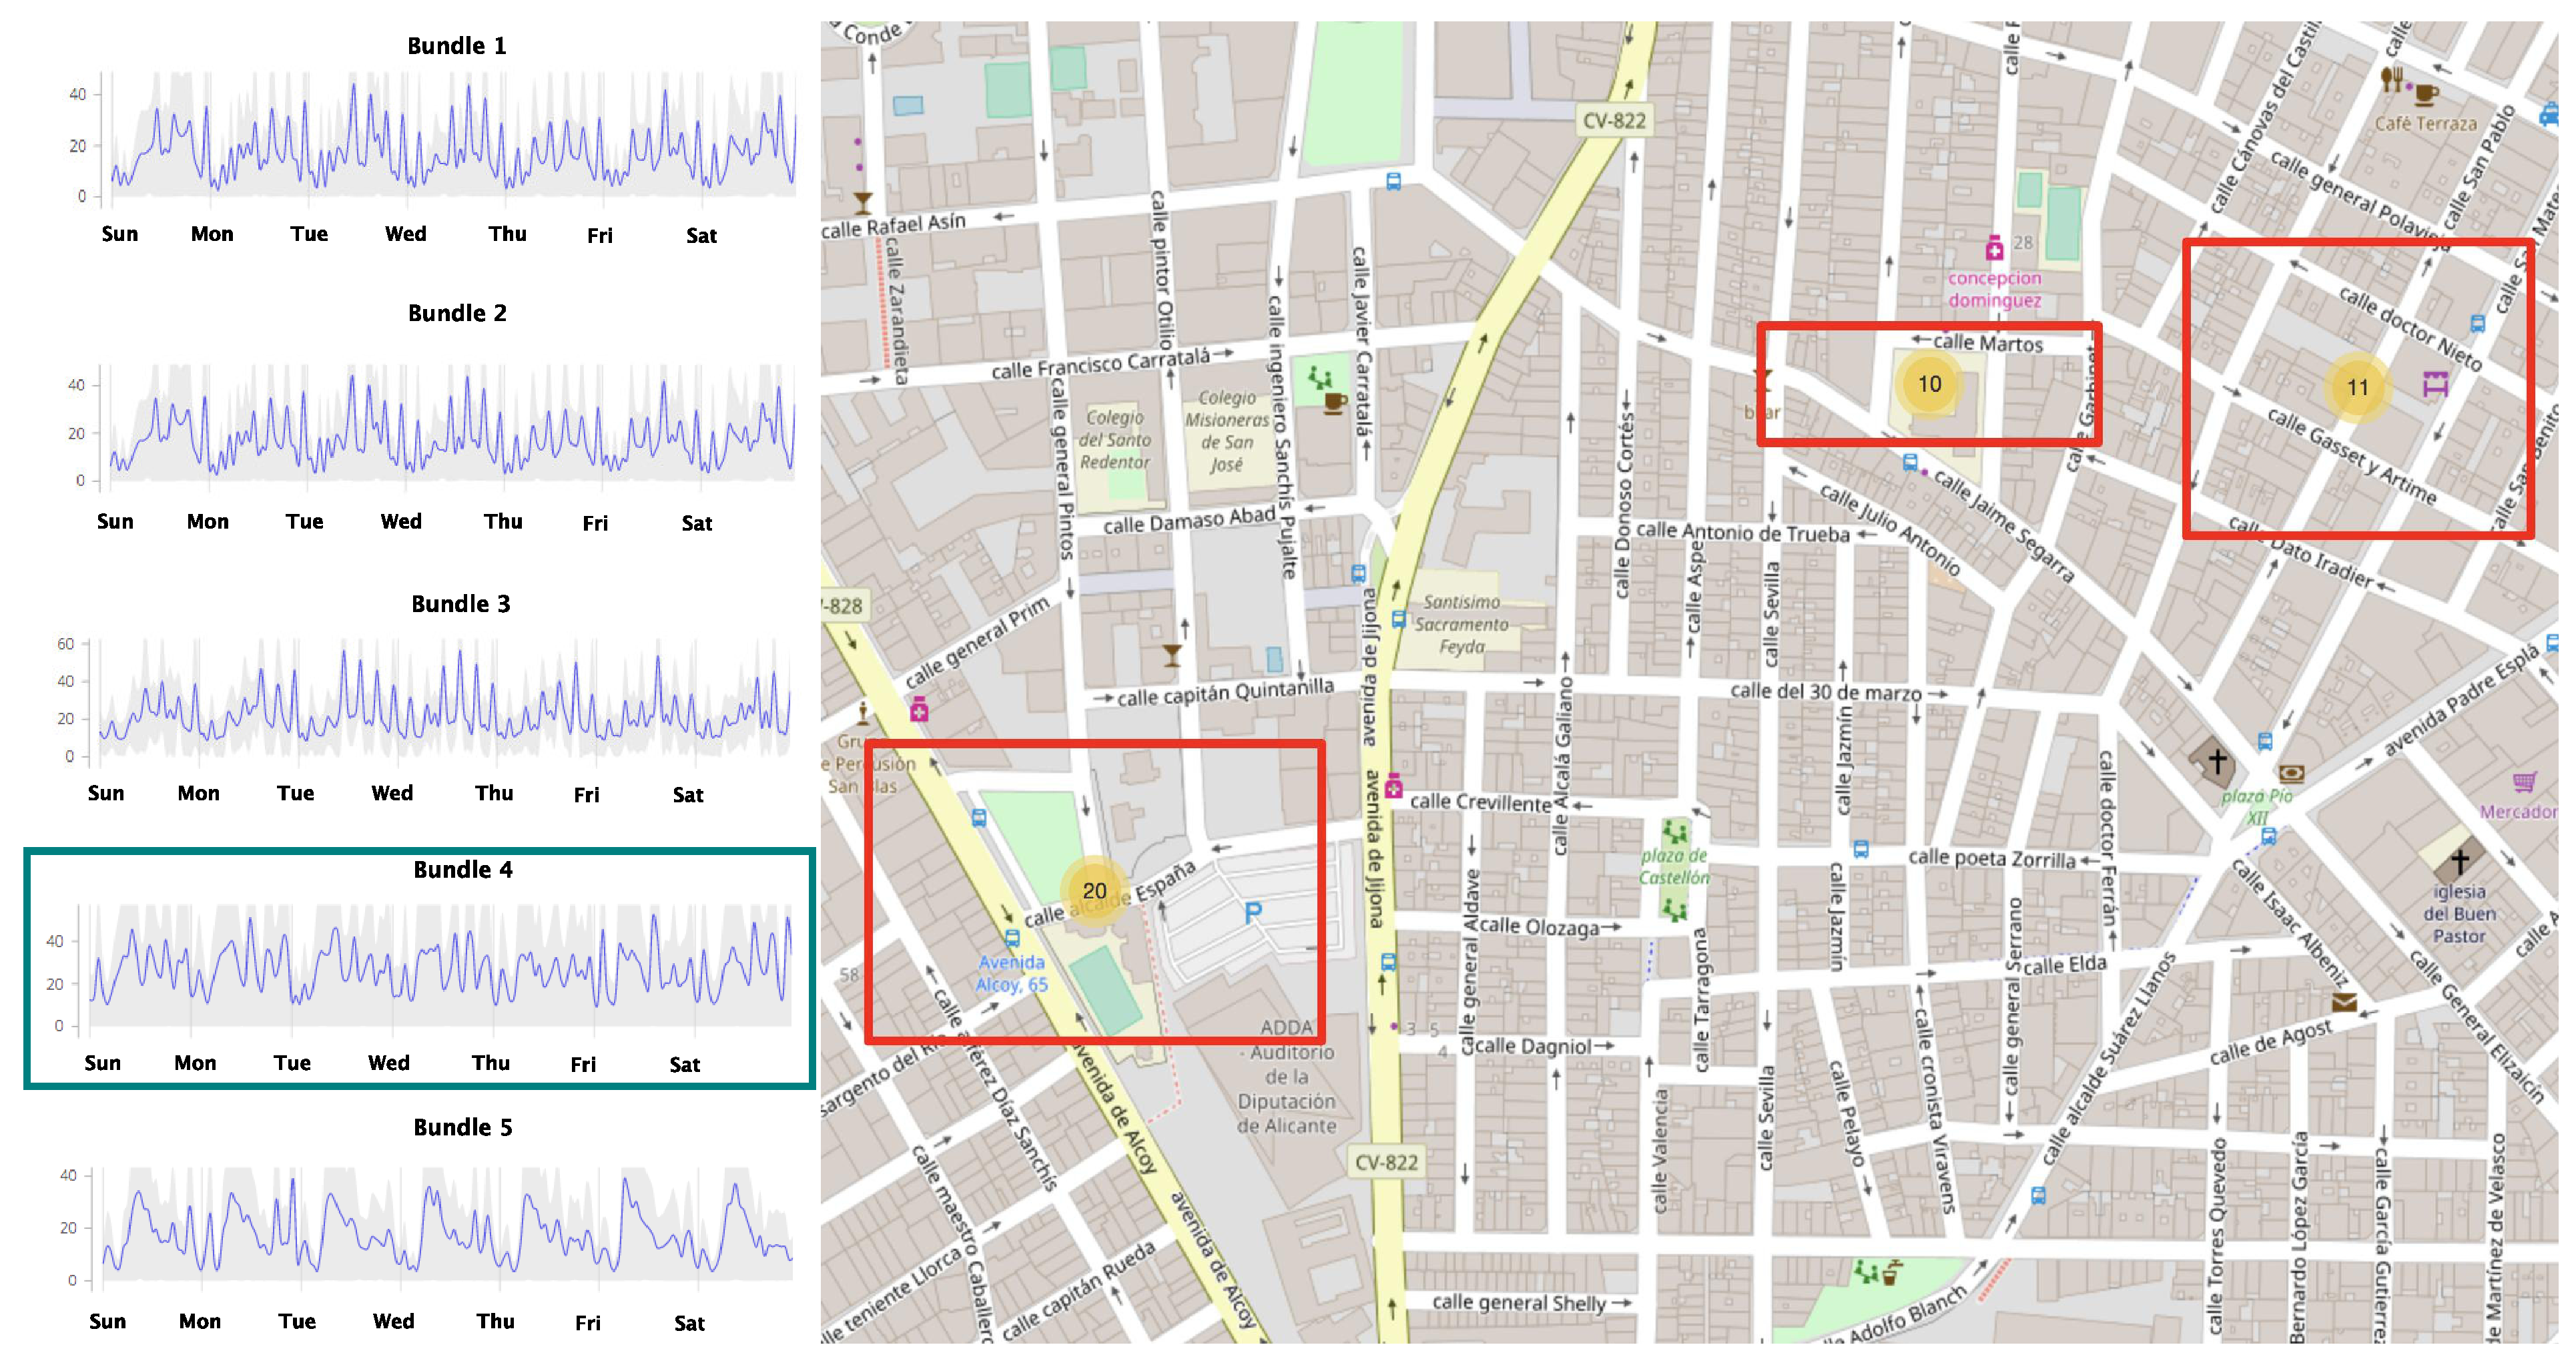
\includegraphics[width=\textwidth]{figures/alicante_btsr_explorer.eps}}
 %\vspace{-7pt}
 \caption{Visualizing water consumption patterns in the city center of Alicante (map scale 1:5000).}
 \label{fig:alicante_example}
\end{figure*}


Figure~\ref{fig:alicante_example} shows an example of such visualization using the water dataset. The depicted area is in the center of Alicante, in the most densely populated zone of the city. In this example, \texttt{Bundle 4} is selected (indicated with a green colored frame) and the relevant MBRs are shown on the map (using red colored frames). This indicates that inside each depicted MBR there exists a specific number of geolocated time series that have been clustered to the chosen bundle. As mentioned, each geolocated time series in this dataset represents hourly water consumption of a household across one week. Different consumption behaviors have been grouped together and a daily pattern for each bundle can be noticed which is due to the Circadian rhythmic way that people consume water \cite{aschoff1965circadian}. The rather large number of geolocated time series in the bundle, considering the zoom level and the extent of the MBRs, intuitively suggests that neighboring families tend to have similar water consumption behavior. 


Figure~\ref{fig:nyc_example} illustrates another example, this time using the taxi dataset in New York City. This dataset is significantly larger, and the zoom level selected in this example is lower (a larger geographic area is visible), hence the MBRs contain a larger number of time series. In this figure, we choose \texttt{Bundle 1}, which represents the rather quieter taxi dropoff zones in Manhattan, as the total number of dropoffs there is rarely over 60 during any hour of the week. In this example, there is also a clear daily routine in all bundles, with the dropoffs reaching a local maximum twice per day, suggesting the rush hours in New York City, when people commute to and from their work. In almost all bundles, the daily pattern is significantly different on Saturdays and Sundays, which confirms the intuition that during weekends people do not tend to commute in a routinely fashion. Overall, such visual representations of information digested from massive time series data can easily catch users' attention to important phenomena and ongoing trends, confirming the usefulness of our approach.

\begin{figure*}[ht]
 \centering
 \fbox{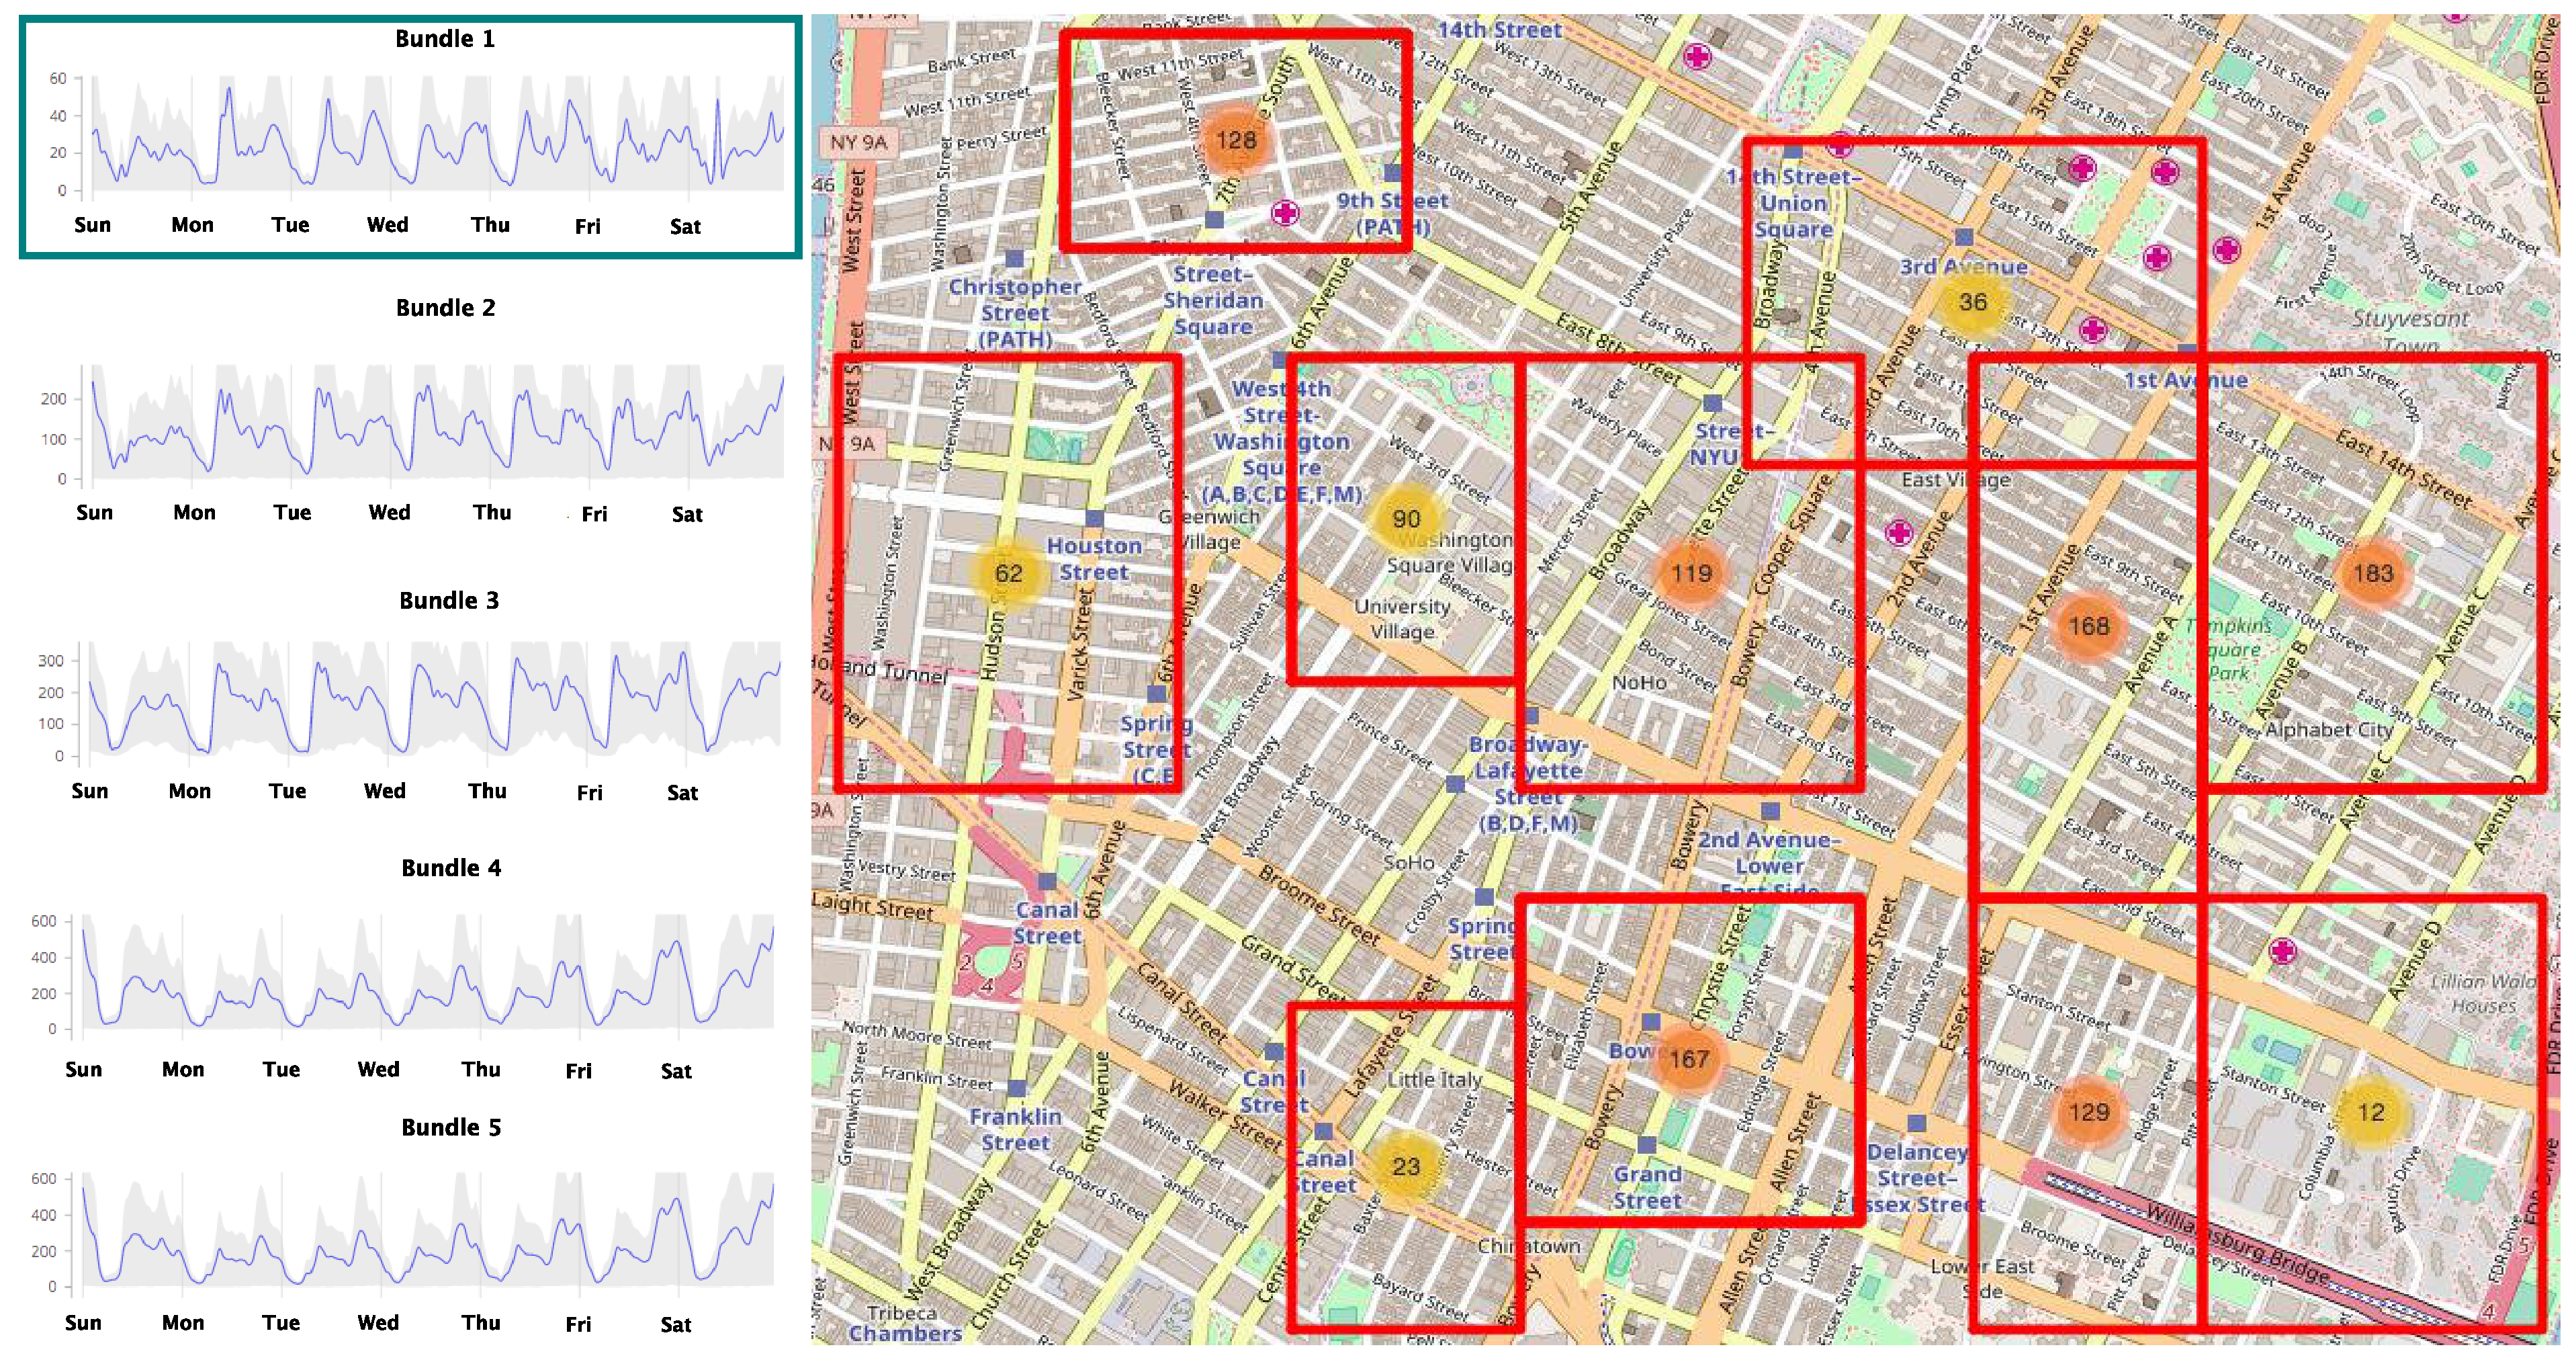
\includegraphics[width=\textwidth]{figures/nyc_btsr_explorer.eps}}
 \vspace{-7pt}
 \caption{Visualization of taxi dropoff patterns in Manhattan, NYC (map scale 1:10000).}
 \label{fig:nyc_example}
\end{figure*}

\vspace{-5pt}
\subsection{Performance Results}
\label{subsec:benchmarking}

In order to evaluate the performance of our approach on larger datasets, we built the index using the synthetic dataset and examined its response time for different zoom levels on the map. Since this is intended as an interactive application, where the summarization method is triggered as soon as the user moves the map, response times must be adequately small. Ideally, the response time should be in the order of milliseconds. In our method, this is facilitated by the fact that the search along a path stops once it encounters a node whose MBR is contained in the actual map extent (rectangle). In this experiment, we measure the response time for different zoom levels, since zooming-in requires deeper traversal of the \btsr index in order to locate the relevant nodes. We use map scales to indicate the different zoom levels. 

%Table~\ref{tab:evaluation} lists the results for different zoom levels. \snote{[Not sure whether the information in the table (regarding node accesses) is really interesting, given that this paper is about visualization and not the index itself. I would prefer to have a plot (line or bars) with zoom level on x axis and execution time on y axis. Also, for the zoom level, it would be perhaps better to specify it by means of the size of the query area (instead of high, medium, etc.)]}

%\snote{ {\bf CHECK:} Remove the grid from the plot in Figure~\ref{fig:zoom} ? On the $y$-axis, 0 should be at the same level as the $x$-axis. Rename label for $x$-axis to `Map scale'.}


Figure~\ref{fig:zoom} depicts traversal costs for different map scales over the areas covered by the three datasets. More specifically, the water and synthetic datasets cover the area of the city of Alicante, Spain, whereas the taxi dataset the wider metropolitan area of New York City. Response time in all cases is equal or lower than one second, which makes this method suitable for interactive visualization. The synthetic dataset, due to its very high density is significantly slower than the rest, however still the results are obtained in less than a second. The response for the water dataset is almost instant due to its small size and very low density.

Initially, in all cases, at the largest scale, the visible area of the map contains all the time series in the dataset, thus it only has to retrieve information from the root of the index. Then, as we zoom in, more nodes have to be visited, as the MBRs of the accessed nodes begin to overlap with the map rectangle and their children have to be retrieved. The worst case for the synthetic dataset is at scale 1:5000, which roughly corresponds to a large neighborhood of the city, where many time series are located. For the taxi dataset, the worst case is at 1:20000, which corresponds to the wider Manhattan area and then the response time gradually drops due to the lower dataset density. The number of nodes accessed in each case is proportional to the response times, ranging from one node (the root) in case of the smaller map scale (all city) up to 165 at scale of 1:5000 for the synthetic dataset, one up to 53 for the taxi dataset and one up to 15 for the water dataset. Interestingly, fewer node accesses are required in all cases at the very large scale of 1:500, since the respective small map area overlaps with fewer nodes and most of the search space is pruned. 

Consequently, we deem that our method performs adequately fast even against a heavily dense synthetic dataset, where a large number of time series are contained within a small area.

%\snote{{\bf CHECK my comment:} We expect a much better performance in typical real datasets with millions of time series; we plan to make more tests, although it is hard to acquire such datasets. }

%\vspace{-5pt}
\begin{figure}[!t]
 \centering
 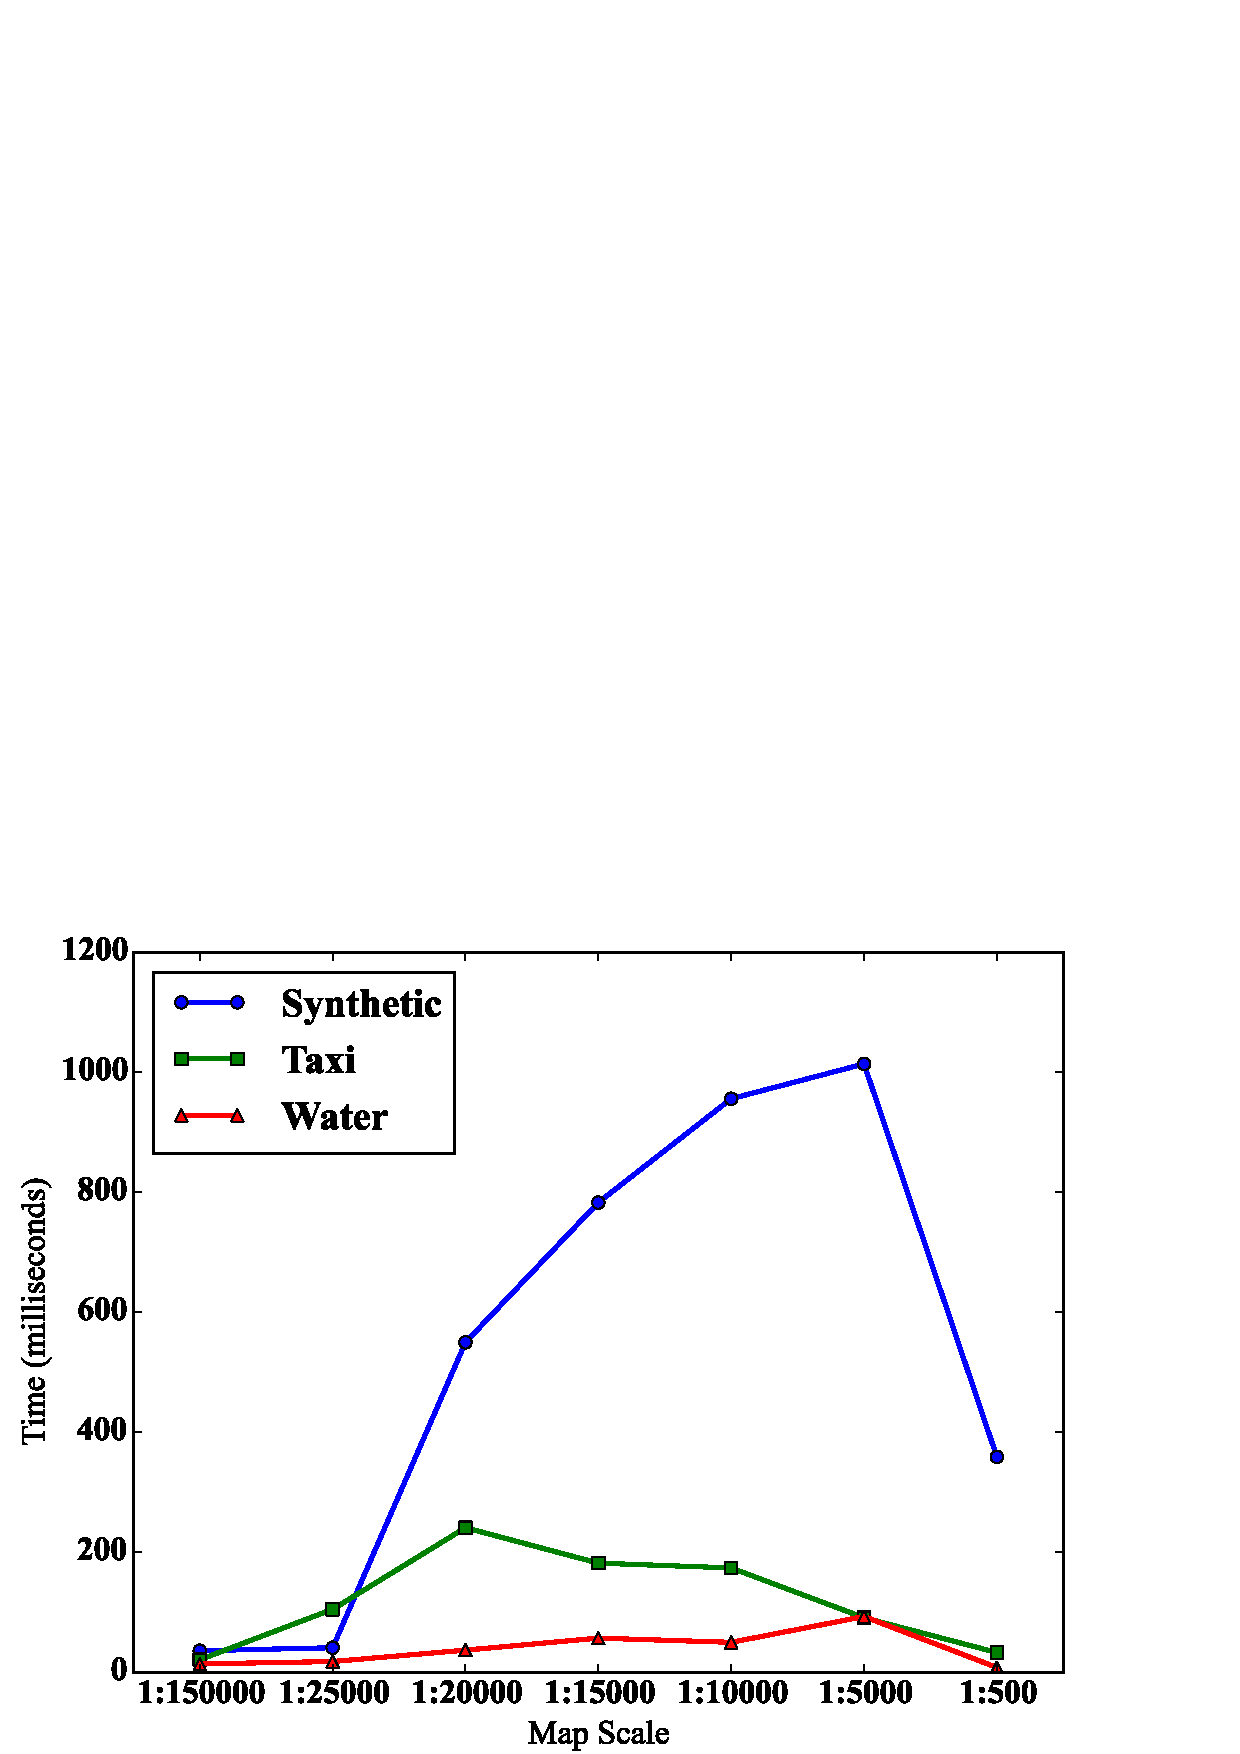
\includegraphics[width=\columnwidth]{figures/zoom_levels.pdf}
 \vspace{-15pt}
 \caption{Execution time for different map scales.}
 \label{fig:zoom}
\end{figure}
%\vspace{-5pt}

% \begin{table}[!h]
% 	\centering
% 	\caption{Performance of the traversal algorithm at different zoom levels.}
% 	\vspace{-10pt}
% 	\begin{small}
% 	\centering
% 	\resizebox{\linewidth}{!}{
% 	\begin{tabular}{lcccccc}
% 	\hline
% 	\multirow{2}{*}{Zoom level} & Execution time & Node & Inner node & Leaf node \\
% 	 & (milliseconds) & accesses (\%) & accesses & accesses \\
% 	\hline
% 	High & 120 & 0.00019 & 13 & 0\\
% 	Medium high & 154 & 0.00028 & 19 & 0 \\
% 	Medium & 495 & 0.0012 & 76 & 0\\
% 	Medium low & 662 & 0.0013 & 93 & 0 \\
% 	Low & 410 & 0.000015 & 1 & 0\\
% 	\hline
% 	\end{tabular}}
% 	\end{small}
% 	\label{tab:evaluation}
% \end{table}